% !TeX root = ../main.tex

\chapter{问答网站智能合约实证研究方法}\label{citations}
\section{问题分析与解决思路}
在本章中,本文对StackOverflow上的代码片段进行安全性与低效性的研究,更具体的,对于漏洞与低效模式是否存在扩散情况,也进一步的进行研究。
这些研究问题的具体实验将在第四章介绍,对于研究问题的设置与实验方法则在本章介绍。

\subsection{问题分析}
对问答网站上代码片段的漏洞分析由来已久,并且研究\cite{fisher1}\cite{dicos}表明问答网站代码片段存在漏洞,可用且危险的代码片段伴扩散到现实环境如Github或谷歌手机应用。但目前的情况是,一方面,对于智能合约的研究已经兴起,而对它在问答网站上的代码片段的潜在漏洞尚无研究;Chen等\cite{define_defect}通过阅读StackOverflow智能合约代码片段定义了20种缺陷,然而这些缺陷到底以什么形式在什么程度下存在于StackOverflow中,以及它们在现实环境中的存在情况尚无研究。

另一方面,智能合约是基于区块链,与虚拟货币高度相关的,这意味着智能合约的漏洞也有所不同,这不仅仅是漏洞类型,漏洞危害程度不同,还有一种全新的基于区块链出现的运行损耗——Gas的高消耗代码模式。在目前的主流的智能合约漏洞与Gas低效模式相关研究中,已经出现了相当多的工具以供使用\cite{Mythril}\cite{Slither}。

智能合约与传统语言迥异,它无法简单的复制传统语言在相关研究下的方案,轻易的获取结果;Felix等\cite{fisher1}通过基础工具PPA\cite{partial_java}补全代码获取字节码的方式进行研究,根据目前存在的加密API方面的糟糕代码模式,它定义了多种漏洞。在问答网站智能合约中,目前并没有解决代码无法编译的基础工具,然而检测工具大多基于编译后的字节码,这使得代码片段无法编译的问题更加重要。

\subsection{解决思路}
当前情况下,没有基础工具的问答网站智能合约实证研究可以通过代码克隆获取智能合约代码片段的漏洞与Gas低效模式。

运用第二章提出的基于抽象语法树的代码克隆方法,本文能找到一个来自StackOverflow的代码片段中函数或者合约的相似克隆对,这个函数或者合约与来自Etherscan的开源智能合约的函数或者合约相匹配;它们在语法上一致,在语义上相似,因此当开源智能合约中找到了某个错误时,本文通过这种相似克隆关系,将错误根据行信息定位到来自StackOverflow的代码片段上。

\begin{figure*}[htbp]
\centering
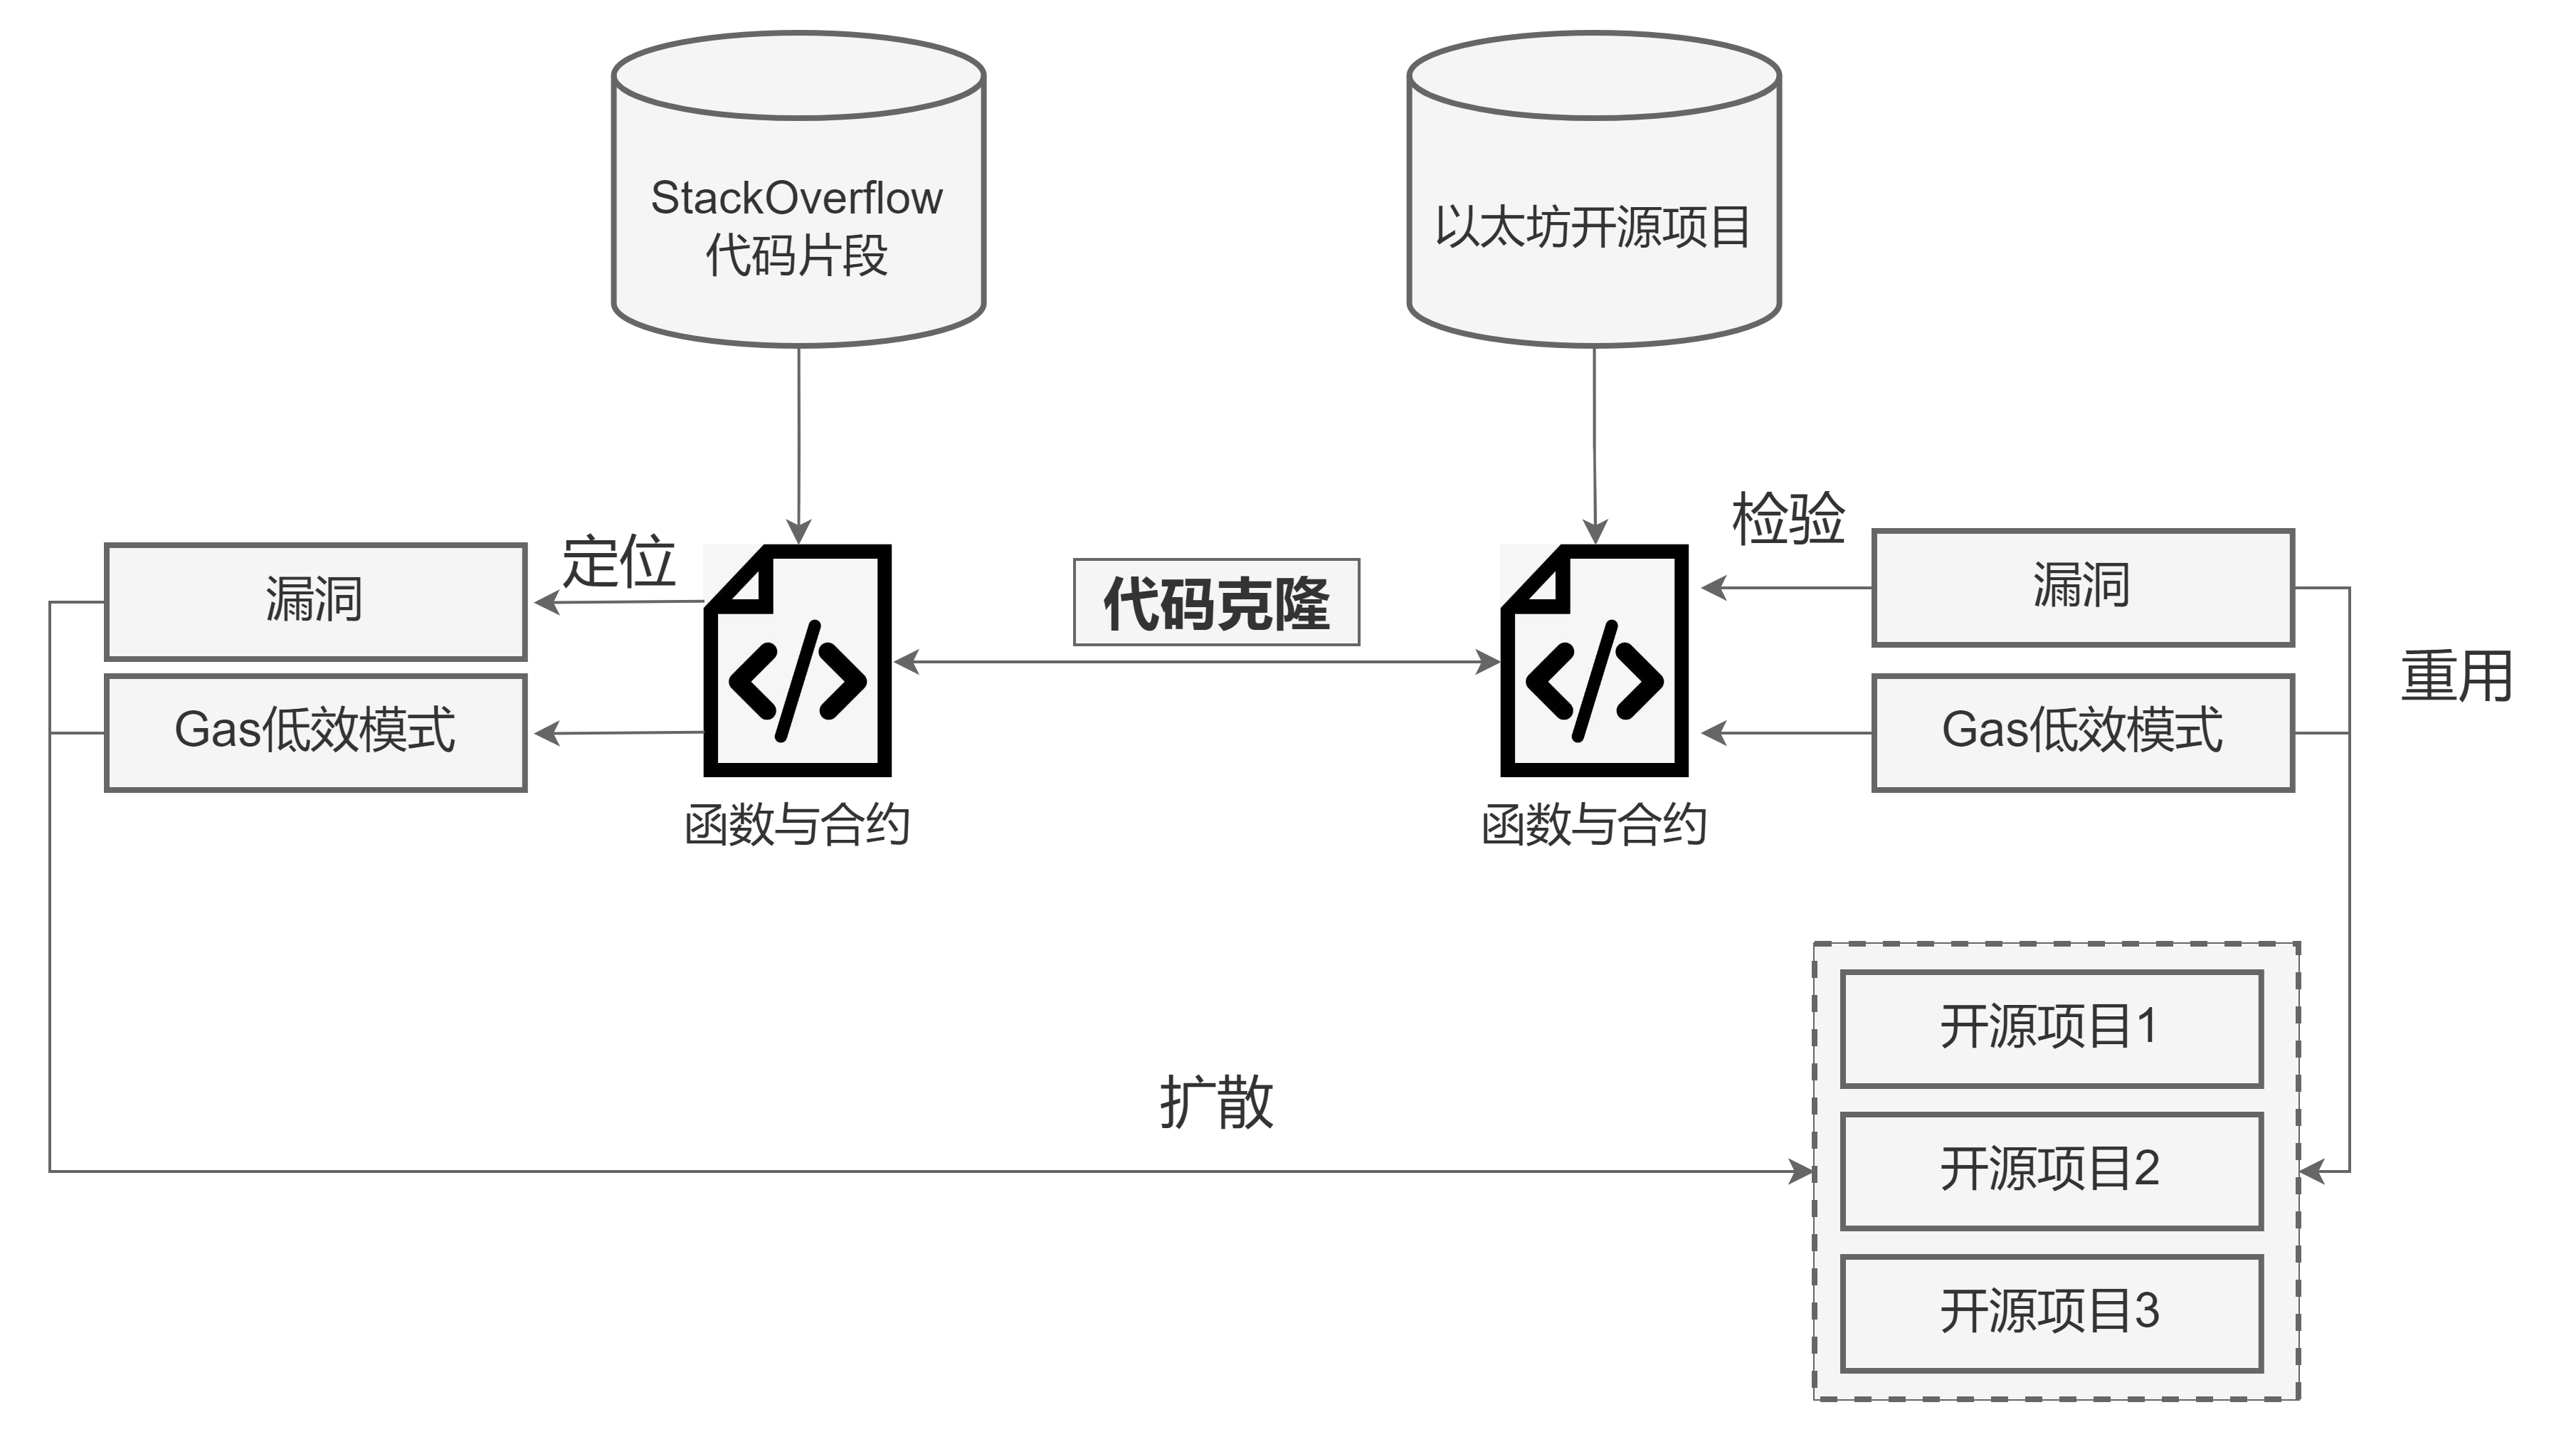
\includegraphics[width=0.8\textwidth]{figures/chapter3Overview.png}
\caption{第三章方法简介}
\captionsetup{font={footnotesize}}
\label{chapter3Overview}
\end{figure*}

本文的方法步骤简要如下所示,方法简介如图\ref{chapter3Overview}所示:
\begin{itemize}
    \item \textbf{使用代码克隆方法}:使用基于抽象语法树的代码克隆方法,找到每个来自StackOverflow的代码片段中合约或者函数的匹配对,这些匹配对遵循语法相似,语义相似的原则。
    \item \textbf{工具选择与处理}:对开源项目库中所有的完整开源合约项目,本文通过阅读相关文献,挑选较新且主流的针对智能合约漏洞与Gas低效模式的检测工具;关于漏洞,本文对它们的结果进行整合,统一成几种常见类型;关于Gas低效模式,本文仅使用了一个工具,这是因为Gas低效模式的检测工具开源较少,并且工具与工具之间检测范围差别较大。
    \item \textbf{漏洞与Gas低效模式定位}:对于一个完成了漏洞与Gas低效模式检测的开源项目,本文根据它的匹配情况,使用行信息找到它能与StackOverflow匹配的多段函数或者合约,如果漏洞与Gas低效模式同样存在于这些函数或合约,本文就认为漏洞与Gas低效模式可以映射到StackOverflow的代码片段中。
    \item \textbf{漏洞与Gas低效模式扩散}:完成了对StackOverflow的漏洞与Gas低效模式的检测后,本文希望找到这些StackOverflow的漏洞与Gas低效模式是否扩散到了现实的智能合约中,因此本文对现有的开源项目进行软件重用分析,经过预处理步骤,本文检测StackOverflow代码片段匹配的完整开源项目合约的重用情况。
\end{itemize}

% 本文会在每节中介绍这个章节下对应的研究问题以及它的设置原因与方案。

% 在章节\ref{bugAnalysis}中,本文介绍了对应第四章中研究问题4,也就是“StackOverflow的智能合约或函数中有多少漏洞?”的方案。

% 在章节\ref{gasAnalysis}中,本文介绍了对应第四章中研究问题5,也就是“ StackOverflow 的智能合约或函数中有多少Gas低效模式?”的方案。

% 在章节\ref{proAnalysis}中,本文介绍了对应第四章中研究问题6,也就是“这些漏洞与Gas 低效模式在真正的智能合约中的普遍程度如何?”的方案。

\section{\label{bugAnalysis}问答网站智能合约漏洞分布}

通过使用代码克隆方法,本文能够找到了StackOverflow 中的合约或函数与开源项目库的合约或函数的匹配。接下来,本文对开源项目进行漏洞与Gas低效模式的检测。如果一个漏洞在开源项目库存在匹配的部分中,来自 StackOverflow 的代码片段也就能找到相应漏洞。本文使用 SmartBugs\cite{smart_contract},一种集成了多个检测工具的漏洞检测框架进行错误检测。

\subsection{SmartBugs介绍}
为了发现智能合约自动分析工具,SmartBugs通过搜索学术文献\cite{toolSurvey}和互联网上寻找其他工具,扩展了他们的工具列表;其次,并非所有确定的工具都很适合SmartBugs的研究,只有符合以下四个标准的工具被纳入SmartBugs的研究。

\begin{itemize}

\item \textbf{可用和 CLI(Command Line Interface)(标准 1)}:该工具公开可用,支持命令行调用(CLI)。

\item \textbf{兼容输入(标准 2)}: 该工具将智能合约作为输入。这就排除了只考虑EVM字节码的工具。

\item \textbf{仅源代码(标准 3)}: 该工具只需要合约的源代码就可以能够运行分析。这就排除了需要测试套件或带有断言注释的合约的工具。

\item \textbf{漏洞发现(标准 4)}: 该工具可以识别合约中的漏洞或不良做法。这排除了部分只构造诸如控制流图这样的工具。

\end{itemize}

SmartBugs发现了9个符合上述纳入标准的工具。\ref{tool_select}给出了被排除和包含的工具,对于被排除的工具,它还显示了它们的排除原因。

\begin{table}[htbp]
\begin{footnotesize}
\centering
\begin{tabular}{@{}ccc@{}}
\toprule
 & 选择标准      & 违反标准的工具          \\ \midrule
\multirow{4}{*}{排除工具(26)} & 可用和CLI(标准1) & Ether, Gasper, ReGuard, Remix, SASC, sCompile, teEther, Zeus                                                                      \\
 & 兼容输入(标准2) & MadMax, Vandal   \\
 & 仅源代码(标准3) & Echidna, VeriSol \\
                        & 漏洞发现(标准4)   &\tabincell{c} { contractLarva, E-EVM, Erays, Ether\.splay, EtherTrust, EthIR, FSolidM,\\ KEVM, Octopus, Porosity, rattle, Sol\.graph, SolMet, Solhint} \\ \midrule
可用工具(9)                   & \multicolumn{2}{c}{HoneyBadger, Maian, Manticore, Mythril, Osiris, Oyente, Securify, Slither, Smartcheck}                                       \\ \bottomrule
\end{tabular}
\caption{根据SmartBugs的纳入标准,排除或纳入的分析工具}
\label{tool_select}
\end{footnotesize}
\end{table}

对于候选的工具,简短介绍如下所示。

Oyente\cite{oyente}是首批智能合约分析工具之一。Oyente使用EVM字节码上的符号执行来识别漏洞。

HoneyBadger\cite{honey}是由卢森堡大学研究人员开发的基于Oyente的工具,它使用符号执行和一组启发式方法来精确定位智能合约中的蜜罐。蜜罐是一种特殊的智能合约,它在设计上看似存在明显的缺陷,允许任意用户从合约中通过预先存储一定以太币的方式来偷走以太币,然而当用户将一定数量的以太币转移到合约中,却将无法取出。

Maian\cite{maian},也基于Oyente。Maian寻找自杀合约,或者可以存储以太币但没有支付功能的合约。

Manticore\cite{manticore}使用符号执行在EVM字节码中查找执行路径,以找到重入漏洞。

Mythril\cite{Mythril}依赖于对EVM字节码的并行分析、污染分析和控制流检查来缩小搜索空间,它能检查包括重入、时间戳操纵等多种漏洞。

Osiris\cite{Osiris}是由卢森堡大学研究人员开发的,它扩展了Oyente,用于检测智能合约中的算术错误。

Securify\cite{securify}使用数据求解器静态分析EVM字节码,以推断有关合约的相关和精确的语义信息。然后,它检查数据一致性和特定的字节码模式,以捕获漏洞。

Slither\cite{Slither}是一个静态分析框架,它将智能合约源代码转换为一个称为Slither的中间表示,并应用已知的程序分析技术,如数据流和污染跟踪来提取和细化信息。

Smartcheck\cite{smartembed}是一个静态分析工具,用于查找漏洞模式和错误的编码实践。它对源代码进行词汇和语法分析。

\subsubsection{漏洞工具性能分析}

SmartBugs使用了他们收集的69个完整项目数据集。SmartBugs进行漏洞工具性能分析所采用的方法如下:
\begin{itemize}
    \item [1.]SmartBugs在69个合约上执行了9个工具。
    \item [2.]SmartBugs将这些工具检测到的所有漏洞提取到一个Json文件中。
    \item [3.]SmartBugs将检测到的漏洞映射到一类漏洞中。为了实现这项任务,SmartBugs将已检测到的所有漏洞类型标记为10个DASP(Decentralized Application Security Project)类别之一。例如,Oyente检测到一个叫做整数溢出的漏洞,SmartBugs将其归类到图\ref{DASP}中的类别Arithmetic。SmartBugs总共确定了141个漏洞类型。
\end{itemize}

实验表明,Mythril工具在这9个工具中具有最好的准确性。此外,Mythril是检测最多不同类别(5个类别)的工具。SmartBugs还发现,Slither是唯一能够识别5个类别中的8个漏洞。尽管Mythil的结果不错,但Mythril它的功能不足以取代所有的工具:通过结合所有工具的检测能力,SmartBugs成功地检测到了42\%的漏洞。

综上所述,Mythril本身的检测准确率较高,而Mythril和Slither的结合可以检测8种类别的结果。本文还观察到 Osiris 在算术 漏洞下具有很高的性能,所以本文也选择了 Osiris。

\subsection{漏洞归类}

不同的工具检测不同的漏洞。本文使用的3个工具总共包含55种漏洞。出于统计与解释结果的目的,有必要根据漏洞的归属类型将它们进一步分类。

 DASP\footnote{\url{https://dasp.co/}}中提出的分类法用于描述以太坊智能合约的漏洞。对于工具中的每个漏洞类型,可以根据工具本身的描述和漏洞类型的威胁等级进行分类,DASP的类型如\ref{DASP}所示。

\begin{table*}[htbp]
\centering
\begin{footnotesize}

\begin{tabular}{@{}lll@{}}
\toprule
{\color[HTML]{494949} 分类} & {\color[HTML]{494949} 描述}                               & {\color[HTML]{494949} 发生层面} \\ \midrule
Reentrancy                      & 重入的调用函数导致难以预测的运行结果 & Solidity                     \\
Access-Control                  & 不合理的使用函数modifiers或者使用tx.origin          & Solidity                     \\
Arithmetic                      & int变量类型上溢或下溢                                    & Solidity                     \\
Unchecked-Low-Calls         & 没有检查函数调用的返回结果                             & Solidity                     \\
Denial-Service               & 运算耗时过长导致合约无法正常处理请求,也就是Dos攻击   & Solidity                     \\
Bad-Randomness                  & 依赖可以被矿工控制的变量信息生成易受攻击的随机数          & Blockchain                   \\
Front-Running                   & 在一个区块中对同一合约多次调用,结果不同  & Blockchain                   \\
Time-Manipulation               & 矿工操纵时间戳引发错误                           & Blockchain                   \\
Short-Addresses                   & 在EVM层接受错误长度的地址信息        & EVM                          \\ \bottomrule
\end{tabular}
\end{footnotesize}
\caption{DASP分类法}
\label{DASP}
\end{table*}%DASP

其中发生层面指的是由于代码编写错误,导致漏洞发生时,是在哪个运行层面发生错误。如\ref{processOfRun}所示,源代码以Solidity语言编写后,在虚拟机EVM(Etherscan virtual machine)上运行,保留运行结果(也被称为交易),被矿工打包,储存到区块链中。代码的编写错误,会让漏洞在这三个不同层面发生。

如Arithmetic类型的上下溢出漏洞,软件的运行逻辑与结果虽然错误了,然而在EVM层与Blockchain层中,经过上下溢出的某个int变量实际上仍然是正确的。而对于Blockchain层的漏洞,则是由于智能合约是运行在区块链上的,很多时候,一些加密程序需要的随机种子或者对时间戳的引用都要在矿工挖取区块,打包交易时确定;这导致如随机数的生成结果可能被矿工提前获知,因此获利。

smartBugs虽然验证了69个完整项目数据集上的实验结果,但仍然无法验证本文收集数据的有效性,本文使用三种工具作为组合,检测收集到的开源项目后,对每种漏洞抽样五十个漏洞进行检测。检测结果如\ref{bugcheck}所示。

\begin{table}[htbp]
\centering
\resizebox{\textwidth}{!}{%
\begin{tabular}{@{}lllllllll@{}}
\toprule
{\color[HTML]{494949} 漏洞类型} &
  {\color[HTML]{494949} Access-Control} &
  {\color[HTML]{494949} Arithmetic} &
  {\color[HTML]{494949} Denial-Service} &
  {\color[HTML]{494949} Reentrancy} &
  {\color[HTML]{494949} Unchecked-Low-Calls} &
  {\color[HTML]{494949} Front-Running} &
  {\color[HTML]{494949} Time-Manipulation} &
  {\color[HTML]{494949} 总体} \\ \midrule
{\color[HTML]{494949} 正确个数} &
  {\color[HTML]{494949} 44/50} &
  {\color[HTML]{494949} 42/50} &
  {\color[HTML]{494949} 50/50} &
  {\color[HTML]{494949} 38/50} &
  {\color[HTML]{494949} 50/50} &
  {\color[HTML]{494949} 46/50} &
  {\color[HTML]{494949} 50/50} &
  {\color[HTML]{494949} 316} \\
{\color[HTML]{494949} 百分比} &
  {\color[HTML]{494949} 88.20\%} &
  {\color[HTML]{494949} 84\%} &
  {\color[HTML]{494949} 100\%} &
  {\color[HTML]{494949} 75\%} &
  {\color[HTML]{494949} 100\%} &
  {\color[HTML]{494949} 91.60\%} &
  {\color[HTML]{494949} 100\%} &
  {\color[HTML]{494949} 90.28\%} \\ \bottomrule
\end{tabular}
}
\caption{在开源项目上应用工具组合抽样检测结果}
\label{bugcheck}
\end{table}

\begin{figure*}[htbp]
\centering

\includegraphics[width=0.3\textwidth]{figures/processOfRun.png}
\caption{智能合约运行的三个层面}
\captionsetup{font={footnotesize}}
\label{processOfRun}
\end{figure*}

\subsection{漏洞定位}

完成了开源项目的漏洞与Gas低效模式检测后,可获得漏洞与Gas低效模式的行信息,本文根据开源项目中合约或函数的代码克隆对,可以找到开源项目存在代码克隆关系的StackOverflow代码片段。

漏洞工具的检测结果以<漏洞类型, 行信息>的形式返回检测结果,对于一个来自StackOverflow的合约或者函数,本文首先确定它的克隆对对应的来自开源项目的合约或者函数在开源合约中的范围,如合约A在开源项目的第X行到第Y行;其次,对于所有的漏洞,本文寻找存在于这个范围的漏洞,并且记录它们;如果存在多个工具在同一段找到相同类型的漏洞,本文就认为漏洞查找重复,并且进行去重。

\begin{figure*}[htbp]
\centering
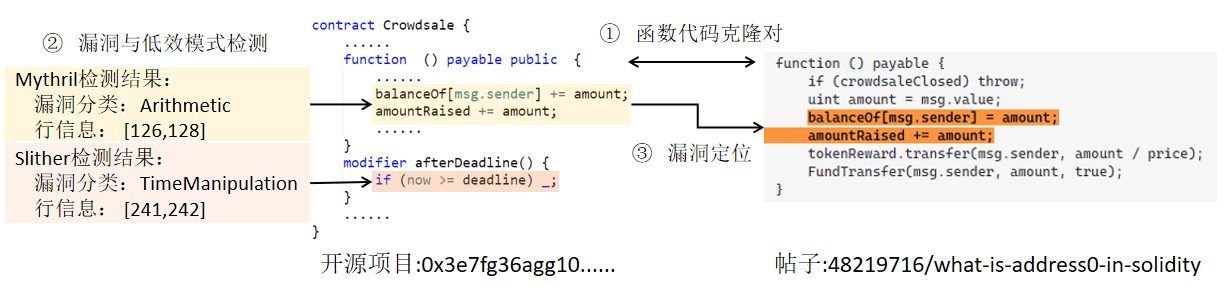
\includegraphics[width=1\textwidth]{figures/locate-example.png}
\caption{漏洞定位的例子}
\captionsetup{font={footnotesize}}
\label{locate-exa}
\end{figure*}

以图\ref{locate-exa}为例,本文先提取开源项目中的函数与来自代码片段的函数,形成函数代码克隆对。其中本文对开源项目进行漏洞检测,根据行信息可以发现来自开源项目的函数存在由Mythril检测的上溢漏洞,本文将其分类为Arithmetic,此时由于这个漏洞出现在一个代码克隆对中,本文将其从开源项目的函数定位到StackOverflow的帖子的函数当中去。至此,本文确定了一个代码片段的漏洞。

\section{\label{gasAnalysis}问答网站智能合约Gas低效模式分布}

在Gas低效模式实证研究部分,本文通过使用Kong等\cite{gasPattern}的工具在开源项目种寻找她们定义的6种Gas低效模式,并且将其映射到StackOverflow的代码片段中。

\subsection{Gas低效模式}

Kong等\cite{gasPattern}从超过25,000篇文章中定义了6个气体低效模式,他们评估天然气效率低下模式的流行程度和经济效益,对超过16万份真实的智能合约进行了实证研究。良好的实验结果表明,52.75\%的合约中至少含有一种低效率气体的模式。如果从合约中删除这些模式,每个合约至少可以节省0.30美元。本文发现目前存在的Gas低效模式的相关研究中\cite{GasChecker}\cite{gasPattern}中仅有该研究开放了源代码,因此本文没有沿用漏洞检测的思路,而是使用单一工具。

本文介绍了该工具GPFinder的六种Gas低效模式,并且说明了本文的处理。

\textbf{Sparse storage}:智能合约以插槽(slots)储存变量。每个插槽占连续的32字节。当一个变量被定义,并且它将要使用的插槽不存在足够大小的空间,那么它将会储存在下一个插槽,当前插槽会因此留下未被使用的空间。插槽越多,智能合约的调用成本越高。如果所有的变量能以正确的顺序进行定义,本文可以使用更少的插槽储存,这能降低智能合约的使用成本。

\textbf{Using smaller values for storage without packing}:当变量无法正常的与其他变量存储在同一个插槽中,他将占据整个插槽,并且使用额外的字节码将变量转换为32字节格式,如int8将会被转换为int256。这个额外的转换操作将导致额外的Gas消耗。

\textbf{Repeat Assignment}:一种常见的变量定义的做法是定义的同时进行初始化,然而这种定义时的初始化值可能很快被后续的赋值覆盖。在字节码层面,本次定义时初始化的字节码的Gas消耗是无意义的。

\textbf{Frequent use of state variables}:读写全局变量比读写局部变量昂贵许多,因为它涉及到操作码SLOAD和SSTORE,它们比其他操作码消耗更多的Gas。特别是,如果读写全局变量的操作是在一个循环中执行的,那么合约消耗的气体会随着循环数量的增加而增加。

\textbf{Without Considering the short-circuiting rules}:短路规则(Short-circuiting Rules)适用于操作符\|\|和\&\&,这意味着在表达式 f(x)\|\| g(y) 中,f(x)运行结果为真时g(y)将不会运行。这意味着,当运行f(x)比运行g(y)消耗更多Gas时,就会产生无意义的Gas损耗。然而,许多开发人员在开发智能合约时并没有考虑到短路规则,而这导致他们的代码消耗了更多的Gas。

\textbf{Inaccurate function visibility}:函数可见性有四种,即public、external、internal与private。public函数可以由所有人访问。external函数只能通过事务进行访问。如果未指定函数的可见性,则默认为即public。可见性为public的函数比可见性为external的函数消耗更多的Gas,因为前者需要将所有的函数输入参数从调用数据复制到内存中,以便函数能够在内部调用。

\subsection{Gas低效模式定位}

与漏洞检测工具类似的,Gas低效模式检测工具也返回行信息,然而由于它的检测与变量关联较大,因此它的返回结果大多包括变量定义与变量调用的行信息,本文对每个模式返回的结果做了如下的不同的处理。
\begin{itemize}

    \item \textbf{Pattern1}: Pattern1能够检测出变量的存储顺序,并且发现它在32比特的插槽中的低效排列顺序,它会返回多段的,低效的全局变量定义段,本文将它视作一整段,并且要求它在克隆对的范围当中。
    
    \item \textbf{Pattern2}: Pattern2能够做到占据可见低于32比特并且将会被储存到单独插槽的变量,如uint8或者int8,一个变量将会返回一行,对于它返回的可能的多行,本文仅需要找到其中一行即可。
    
    \item \textbf{Pattern3}: Pattern3会返回这个变量的定义位置与调用位置,考虑到这个方法既需要确定变量定义时的预先赋值,又需要找到后续的立即覆盖储存的赋值,本文同时使用了两个位置信息。
    
    \item \textbf{Pattern4}: Pattern4返回对变量重复使用的某段代码段的范围与变量的定义位置,然而与Pattern3不同,这个低效模式的问题在于循环中对全局变量的重复读写,而不是对局部变量进行操作,因此本文认为仅需要调用变量的代码段。
    
    \item \textbf{Pattern5}: Pattern5与Pattern4类似,本文不需要知道在一个完整开源项目中,在一个判断条件中的变量原有的值与修改,本文仅需要根据判断条件中逻辑运算符前后的Gas消耗来确定低效模式,本文仅选择了判断条件所在的代码段。
    
    \item \textbf{Pattern6}: Pattern6检测本应该设置为更低耗公开等级的函数而被默认或强制设置为更高消耗公开等级。在本文的方法中,本文要求了“Modifiers”序列的一致,这有助于提高本文方法的有效性。
    
\end{itemize}

GPFinder\cite{gasPattern}对包含六种Gas低效模式的开源项目进行交易重放,对六种Gas低效模式的Gas额外花费进行了估计,由于交易重放受到单一开源项目存在不同交易次数的影响,对于它的检测结果,本文仅使用合约部署时的Gas额外花费,单位为Gwei。

\begin{table}[htbp]
\centering
\begin{tabular}{@{}cccc@{}}
\toprule
\multicolumn{1}{l}{Gas低效模式} & 重放合约个数 & 部署合约额外Gas消耗 & \multicolumn{1}{c}{低效模式Gas消耗估计} \\ \midrule
Pattern1                    & 11,657 & 80,494,110  & 6905.22                         \\
Pattern2                    & 8,810  & 79,077,573  & 8975.89                         \\
Pattern3                    & 2,149  & 12,262,199  & 5706.00                         \\
Pattern4                    & 1,989  & 23,219,821  & 11674.12                        \\
Pattern5                    & 7,442  & 348,897     & 46.88                           \\
Pattern6                    & 3,216  & 29,664,663  & 9224.09                         \\ \bottomrule
\end{tabular}
\caption{Gas低效模式重放实验与Gas消耗估计}
\label{gasg}
\end{table}

完成了对工具返回信息的处理,本文使用与漏洞检测一致的行信息处理漏洞定位问题。

\section{\label{proAnalysis}问答网站智能合约漏洞与低效模式扩散}

在本节,本文对开源项目进行代码重用分析,并且探究来自StackOverflow的错误在现实环境中的扩散情况。本文的做法也是代码克隆,与之前的代码克隆方法,存在以下区别:

\begin{itemize}
    \item 本文检查的是合约层面的重用情况,而并非项目。这是由于完整的项目的重用是极少的,复用他人的合约是更常见的情形。
    \item 本文Hash了所有的节点,而在第二章中,本文仅Hash了三种节点类型。
    \item 预处理步骤本文对于完全重复的项目中来自同一个合约创建者的重复项目,本文进行了删除,而保留来自其他人的重复项目。
    \item 本文制定了不同的重用标准,使用了最长匹配子序列\cite{longestSeries}确定两个开源项目的重用程度。为了保证漏洞与Gas低效模式定位的一致性,本文取了极高的阈值保证漏洞与Gas低效模式定位的一致性。
\end{itemize}

\subsection{序列化}

从Solidity-parser-antlr输出的AST中的每个节点都有一个“Type”节点来表示其语法结构的类型。本文的Hash方法要对所有节点进行Hash;其中对每一个节点,本文都会Hash它的语法结构类型,尤其是它的“Type”节点内的信息。通过前序遍历方式连接其AST中所有节点的哈希值,生成其Token序列,并从其AST的根节点中提取合约的名称。换句话说,在Token化之后,本文获得了从每个合约的名称到每个合约的Token序列的映射。

\subsection{预处理}

预处理的目标是根据合适的标准对开源项目进行重复数据合并。两个项目定义为相同,仅当它们具有相同数量的合约,并且相应的合约具有相同的名称和相同的源代码。当本文尝试使用这个标准删除重复的项目时,本文发现存在大量项目是重复的,这些重复的项目可以被划分为单独的组。因此,对于每一组重复的项目,本文将进一步分析该组包含多少个相同的项目,以及有多少个不同的创建者创建了这些项目。创造者的信息也是从Etherscan中收集到的。有两种情况:(1)很少有创造者创建了大量相同的项目,(2)有大量的创造者分别创建了几个相同的项目。前者的一个例子是,一个项目由2个创建者重复了42,500次。对于后一种情况,大多数项目都是根据合约模板而开发的。许多创建者通过复制这些模板,然后定制初始化参数,在以太坊上发布他们自己的项目。考虑到这两种情况,本文删除它们的创建者的重复项目,也就是说,本文保留每个创建者创建的一个重复项目,而不是每组重复项目中的一个。

\subsection{代码重用检测}

对于来自 StackOverflow 的错误函数,本文还想知道该函数上的错误是否在真实的智能 合约中普遍存在。评估错误扩散的方法是找到包含匹配的合约或者函数的智能合约的重用次数。也就是说,重用的智能合约代码产生的AST序列相同,因此它们有相同的错误。

本文遵循下列原则检测重用。

\begin{itemize}

    \item \textbf{代码克隆}:两个合约的名称和Token序列完全相同。Token序列包含合约的语法信息,而名称通常包含有关该功能的语义信息。本文不仅考虑Token序列,还考虑名称,因为具有相同名称和令牌序列的合约更有可能基于复制和粘贴而被重用。
    
    \item \textbf{重命名}:两个合约具有相同的Token序列,但名称不同。在某些情况下,开发人员可能会根据不同命名规则,而更改重用的合约名称。因此,本文比较了Token序列,以检测可能的代码重用和重命名。
    
    \item \textbf{代码重用与修改}:只有两个合约的名称是相同的,并且这两个合约之间的语法相似性超过了一个特定的阈值,本文才认为是重用。本文在本文中选择的阈值是0.9。
    
\end{itemize}

其中语法相似性的计算根据其Token序列的最长匹配子序列\cite{longestSeries}来衡量的。

\begin{equation}
    similarity = \frac{length(longestSubSeq)}{max_length(tokenSeq_{1}, tokenSeq_{2})}
\end{equation}

%\subsection{最长匹配子序列算法}


此时,对于一个能够匹配StackOverflow中代码片段的某个开源项目,本文即知道它的那些错误存在于StackOverflow,又知道它的复用情况,因此计算它的错误与复用的乘积就能得知StackOverflow代码片段错误的扩散情况。

\section{本章小结}

本章介绍了使用代码克隆检测方法对StackOverflow上的代码片段进行的实证研究。使用来自Durieux等\cite{tool_paper}的Smartbugs与来自Kong\cite{gasPattern}的工具,本文能够获得开源项目下的漏洞与Gas低效模式信息。本文再使用第二章介绍的代码克隆方法将开源项目的合约或者函数中存在的错误映射到StackOverflow的代码片段;对于StackOverflow代码片段上可能造成的错误扩散,本文的做法是使用代码克隆,获取开源合约的重用关系,StackOverflow的代码片段的漏洞来自存在重用情况的开源项目,本文据此计算出代码片段错误的扩散情况。